\documentclass[12pt]{beamer}
%\usepackage{mystyle}

% Since <T>LAPACK does not properly render in LaTeX without putting < in math mode,
%   we define the following command to make referencing it more convenient
\newcommand{\tla}{$<$T$>$LAPACK}

\author{Johnathan Rhyne}
\title{Developing with \tla}

\begin{document}
    \begin{frame}
        \maketitle
    \end{frame}
    \begin{frame}
        \tableofcontents
    \end{frame}
    \section{Developing for \tla}
    \begin{frame}
        \frametitle{Developing for \tla}
        % This will serve as a reminder slide for the users mostly to draw attention to the templating behavior
        As was said before, the codebase for \tla\, is written in header files. This allows us to 
        take advantage of templates!
    \end{frame}
    \section{My project within \tla}
    \begin{frame}
        \frametitle{My project within \tla}
        I worked on some software that was for a fork of \tla. The code can be found here: 
        \url{https://github.com/jprhyne/tlapack/tree/hqr}, which was investigating porting EISPACK hqr
        into the \tla framework. 
    \end{frame}
    \begin{frame}
        \frametitle{My project within \tla}
        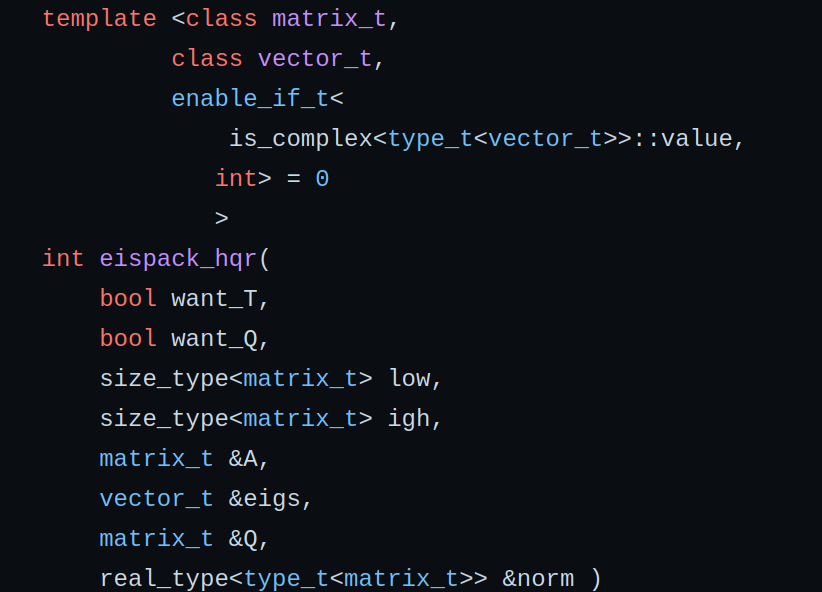
\includegraphics[width=\textwidth]{images/eispackHqr.png}
        % This slide mainly serves as a talking point. Depending on what is talked about previously I may 
        % make this brief and treat it as a showcase of the interface. Or go into some more detail
        % centering around the top part (unsure what will be covered prior to me talking)
    \end{frame}
    \begin{frame}
        \frametitle{My workflow}
        \begin{enumerate}
            \item Write in a language I am comfortable with (C)
            \item Segment the code (create more functions!)
            \item Transcribe a function at a time along with white-box testing
            \item Transcribe the main driver
        \end{enumerate}
    \end{frame}
    \section{Examples of calling code}
    % If they aren't going to talk about Catch2, I will discuss how I used it 
    \begin{frame}
        \frametitle{Examples of calling code}
        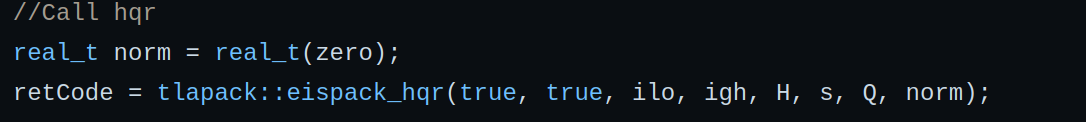
\includegraphics[width=\textwidth]{images/callingHqr.png}
        Looking at the testing files, we don't need to do anything special in order to call our templated
        functions. In fact, it is very similar to how you would use an interface like CBLAS or LAPACKE.

        It's possible to omit the namespace dereference in the function calls, but it is overall not too
        cumbersome to leave it this way and makes it much more clear where functions you are using come from.
    \end{frame}
    \begin{frame}
        \frametitle{Testing our code}
        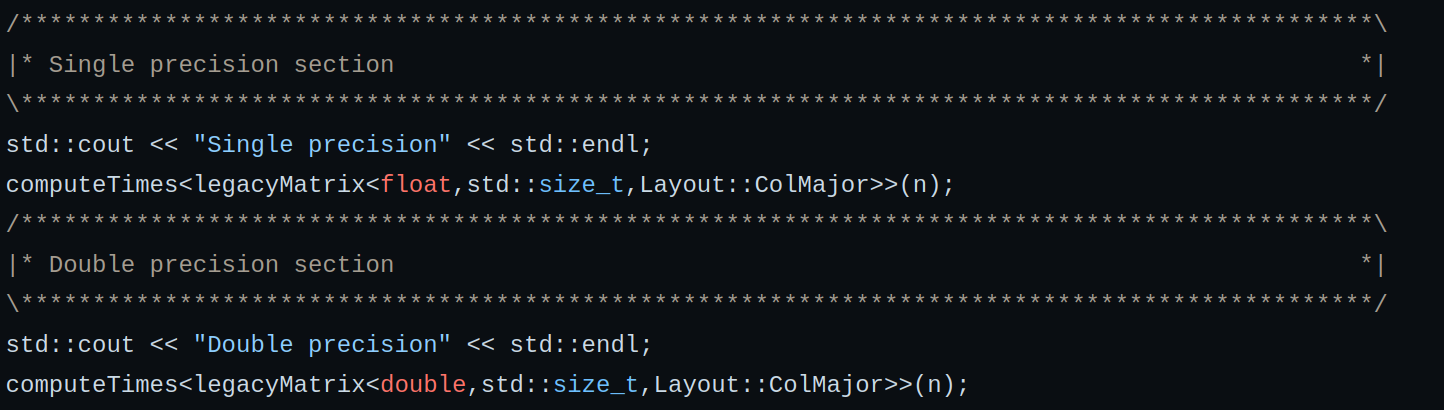
\includegraphics[width=\textwidth]{images/numericalExperiments.png}
        As we can see, when we template, the code that is called can be much simpler and if we are being given
        our data from another source, we don't need to implement any kind of checcking to determine the correct
        call!
        %As far as testing goes, since we are working with a C++ repository, we can take advantage of libraries
        %like Catch2, which facilitate writing test cases in a way familiar to other languages like Java. This
        %means that we an write a single C++ file that will automatically handle reporting errors.
        % Some prefer having all of the tests inside a shell script as this requires less overhead,
        % and doesn't require us to compile our tests. TODO: Ask Julien why he likes this method and add his
        % reasoning
        % One benefit of this is when we are at a large scale, it is much easier to write code in the paradigm of
        % "only tell me where there is a problem, as hearing nothing about a given routine/function
        % implies the functionality works 
    \end{frame}
    \section{Timing of my project}
    \begin{frame}
        \frametitle{Timing of my project}
        We first present the first two ``obvious'' options for our types, single and double precision
        %As was hinted at above, all that we have to change is just the datatype we initialize as and throw
        %it into the same exact function call. This is a little more user friendly than what is done with
        %Fortran LAPACK where we need to call a different function when we use a different data type, and is
        %possible for there to be a bug in a port from double to single 

        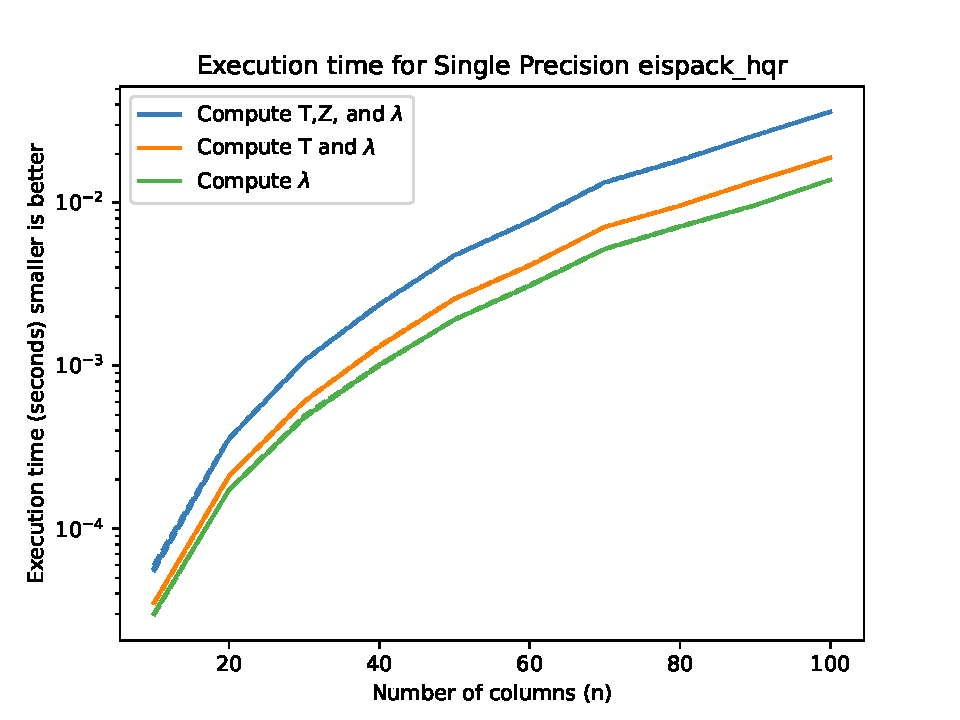
\includegraphics[width=.45\textwidth]{numericalExperiments/eispackHqrTlapackTimeSingle.pdf}
        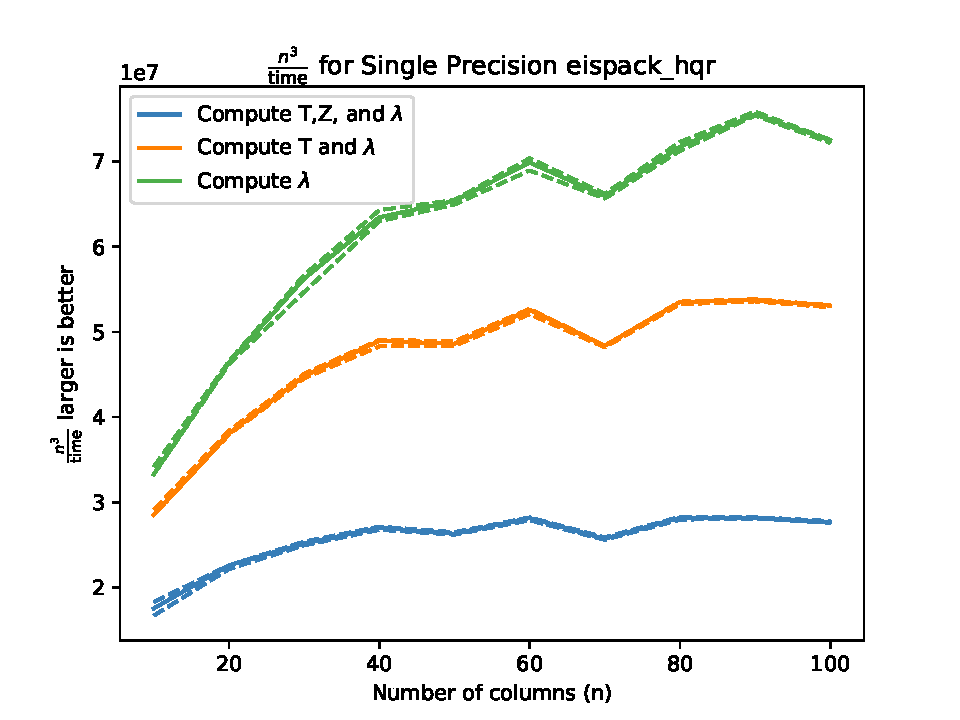
\includegraphics[width=.45\textwidth]{numericalExperiments/eispackHqrTlapackPerfSingle.pdf}
    \end{frame}
    \begin{frame}
        \frametitle{Timing of my project}

        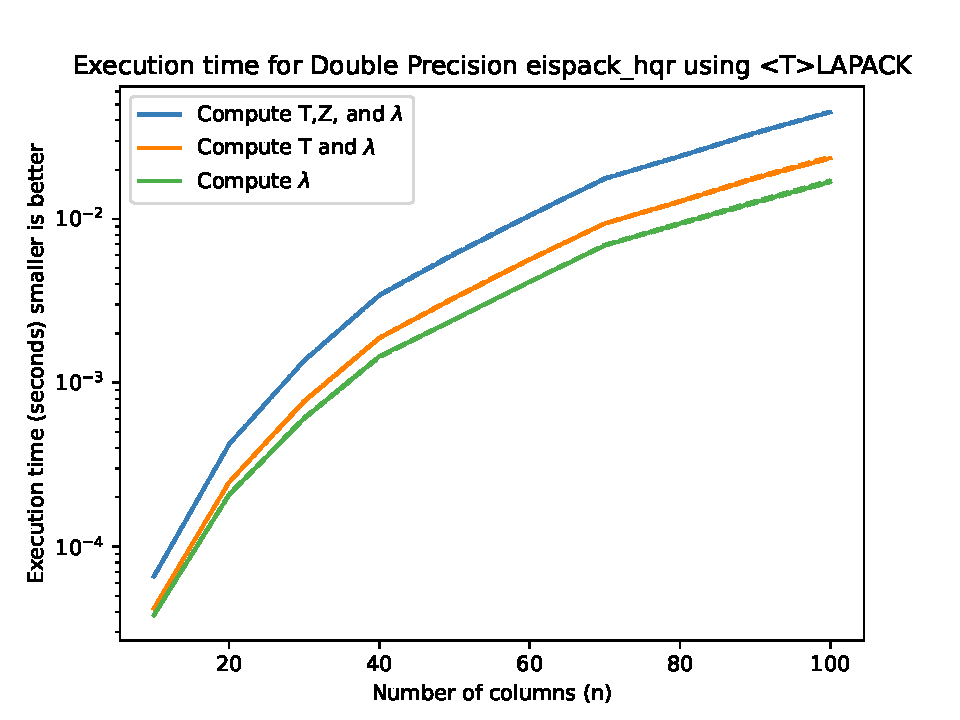
\includegraphics[width=.45\textwidth]{numericalExperiments/eispackHqrTlapackTimeDouble.pdf}
        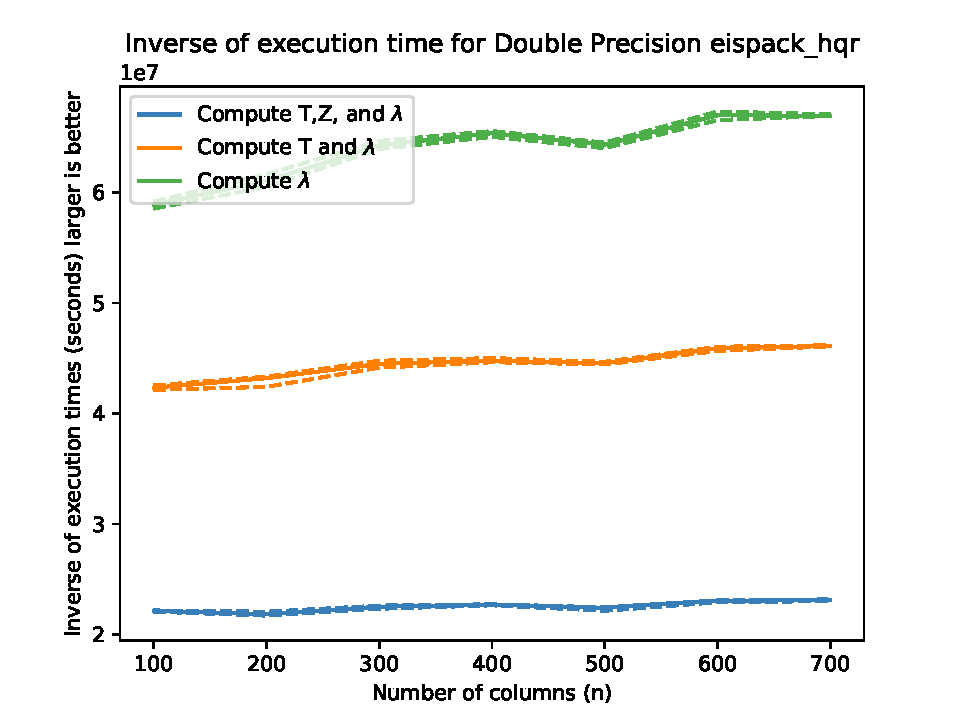
\includegraphics[width=.45\textwidth]{numericalExperiments/eispackHqrTlapackPerfDouble.pdf}
    \end{frame}
    \begin{frame}
        \frametitle{Timing of my project}
        Using multi precision was also just a drag and drop!
        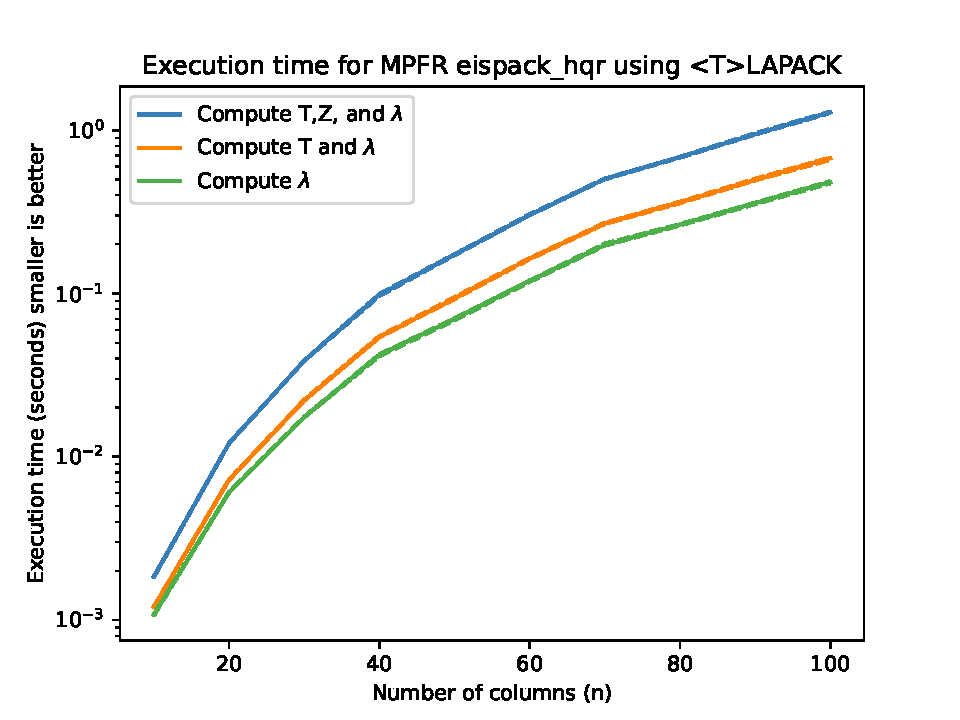
\includegraphics[width=.45\textwidth]{numericalExperiments/eispackHqrTlapackTimeMPFR.pdf}
        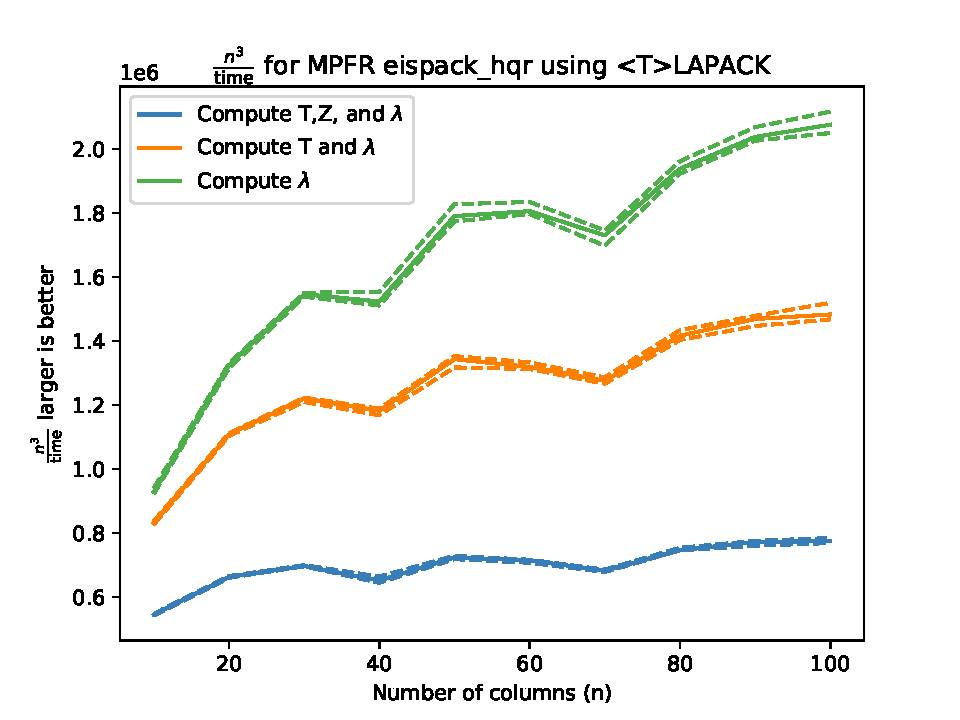
\includegraphics[width=.45\textwidth]{numericalExperiments/eispackHqrTlapackPerfMPFR.pdf}
    \end{frame}
    \iffalse
    \begin{frame}
        \frametitle{Comparing EISPACK to my C++ implementation}
        % This is comparing the results of the C++ and Fortran implementations There is a large difference in execution times. This is something to note.
        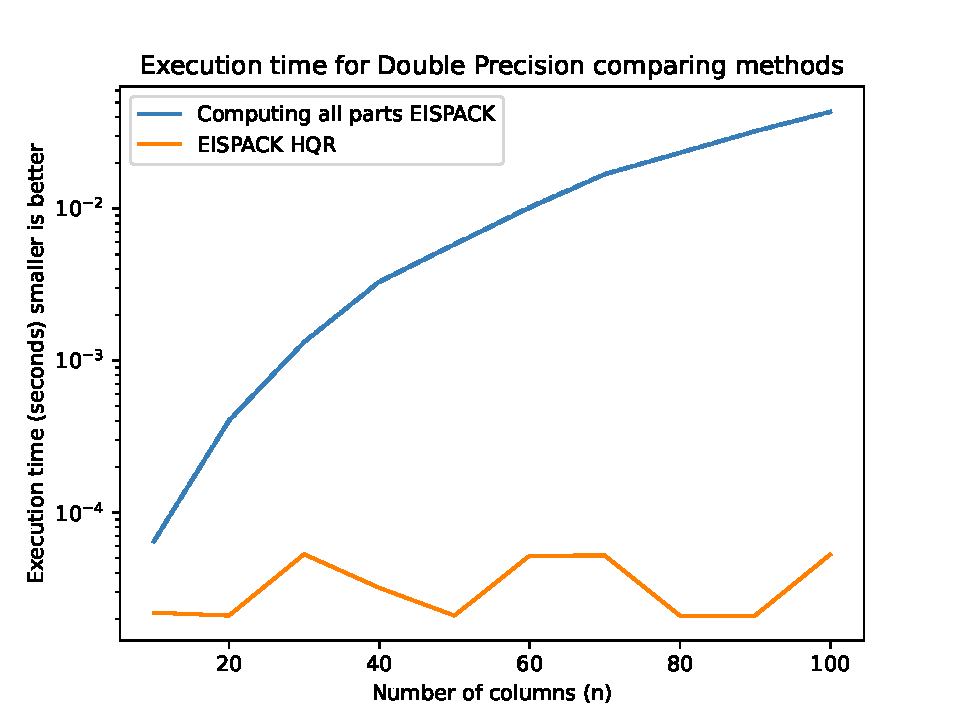
\includegraphics[width=\textwidth]{numericalExperiments/combinedTimeResultsAll.pdf}
    \end{frame}
    \fi
    \section{Differing precisions}
    \begin{frame}
        \frametitle{Differing precisions}
        Some users already use the ease of the templating to use non-standard precisions. For example, this
        user was testing 8-bit floating point arithmetic, and only had to change how data was declared.
        \url{https://github.com/SudhanvaKulkarni123/tlapack}
        % I could not get this working as there are compiler errors pointing to their plugin file, and I'm not
        % an expert when it comes to C++ nor eigen, so I did not figure out if it's an error on my side or not
    \end{frame}
\end{document}
